\documentclass[UTF8]{ctexart}
\usepackage[a4paper,margin=1.8cm]{geometry}
\usepackage{graphicx}
\usepackage{float}
\usepackage{longtable}
\usepackage{array}
\usepackage{xcolor}
\usepackage{fancyvrb}
\usepackage{hyperref}
\setlength{\parindent}{0pt}
\setlength{\parskip}{0.45em}
\begin{document}
\section*{运行时环境完整模拟卷 04（题目与完整解析）}

\subsection*{卷面说明}

\begin{Verbatim}[fontsize=\small,breaklines=true]
考试时间：120 分钟
总分：100 分
说明：本卷独立覆盖存储分配、活动树、栈帧、堆管理、引用计数和跟踪式垃圾回收。
所有调用约定、对象图和内存数据均在题面中给出。
\end{Verbatim}

\subsection*{A 卷题目}

\subsubsection*{一、存储区、活动树与控制栈（20 分）}

某程序的一次执行产生如下动态调用关系，子结点从左到右表示实际调用顺序：

\begin{Verbatim}[fontsize=\small,breaklines=true]
main
├─ f(1)
│  ├─ g(1)
│  └─ g(2)
└─ h()
\end{Verbatim}

1. 静态区、栈区、堆区分别存放什么数据，各举一个例子。 2. 写出本次执行的过程调用顺序。 3. 写出过程返回顺序。 4. 当控制流位于 \texttt{g(2)} 内部时，哪些活动尚未结束；控制栈从栈底到栈顶有哪些活动记录。 5. 说明活动树的前序/后序遍历与调用/返回顺序的关系。

\subsubsection*{二、栈帧布局与调用/返回（20 分）}

程序：

\begin{Verbatim}[fontsize=\small,breaklines=true]
int fun(int a, int b) {
    int c = a - b;
    return c;
}

int main() {
    int i = 100;
    int j = 20;
    int m = fun(i, j);
    return m;
}
\end{Verbatim}

采用如下明确约定：

\begin{Verbatim}[fontsize=\small,breaklines=true]
机器字长 4 字节；栈向低地址增长。
调用者按从右到左顺序压入参数。
call 指令把返回地址压栈。
被调用者执行 push BP；BP=SP；再为局部变量分配 4 字节。
函数返回值放入寄存器 R0。
\end{Verbatim}

1. 写出调用 \texttt{fun(i,j)} 时，从压入第一个参数到完成函数序言的指令顺序。 2. 以 BP 为基准，写出 \texttt{c、旧BP、返回地址、a、b} 的地址偏移。 3. 写出执行 \texttt{c=a-b} 和设置返回值的伪汇编。 4. 写出函数尾声和返回过程。 5. 说明返回后 \texttt{main} 如何得到 \texttt{m=80}。

\subsubsection*{三、堆分配、碎片与分配策略（20 分）}

堆中空闲块按地址从低到高排列，初始大小为：

\begin{Verbatim}[fontsize=\small,breaklines=true]
[6, 14, 8, 20]
\end{Verbatim}

依次发出三个分配请求：

\begin{Verbatim}[fontsize=\small,breaklines=true]
7, 5, 12
\end{Verbatim}

分配时从选中空闲块的低地址端切出所需空间，不考虑对齐和块头开销。

1. 使用 First-Fit，写出每次选中的块及最终空闲块大小。 2. 使用 Best-Fit，写出每次选中的块及最终空闲块大小。 3. 比较两种策略最终最大连续空闲块。 4. 区分内部碎片和外部碎片。 5. 写出存储管理器的空间效率、程序效率和低开销三个评价维度。

\subsubsection*{四、引用计数与不可达环（20 分）}

根和对象引用关系如下：

\begin{Verbatim}[fontsize=\small,breaklines=true]
r1 -> A
r2 -> D
A  -> B
B  -> C
C  -> B
D  -> C
\end{Verbatim}

引用计数只统计根引用和对象字段引用。

1. 写出初始时 A、B、C、D 的引用计数。 2. 执行 \texttt{r1=null} 后，按引用计数规则写出回收过程和新计数。 3. 再执行 \texttt{r2=null} 后，写出回收过程和新计数。 4. 指出此时哪些对象不可达但不能被引用计数回收。 5. 说明跟踪式垃圾回收为什么能回收它们。

\subsubsection*{五、标记-清扫、压缩、拷贝与分代（20 分）}

根和对象图：

\begin{Verbatim}[fontsize=\small,breaklines=true]
R1 -> A        R2 -> F
A -> B, C
B -> D
C -> D, E
D -> B
F -> G
H 无入边
\end{Verbatim}

对象在堆中按地址排列：

\begin{Verbatim}[fontsize=\small,breaklines=true]
对象  起始地址  大小
A     0         2
H     2         2
B     4         3
C     7         2
D     9         1
E     10        2
F     12        1
G     13        2
\end{Verbatim}

1. 从根集出发列出全部可达对象和垃圾对象。 2. 写出标记-清扫两个阶段及清扫结果。 3. 按对象原有顺序向低地址压缩，写出每个存活对象的新起始地址。 4. 说明半空间拷贝回收的 From/To 过程及空间代价。 5. 说明分代回收依据的经验规律，以及记忆集的作用。

\subsection*{B 按考试标准重写答案}

\subsubsection*{一、存储区、活动树与控制栈答案}

\paragraph*{1. 静态区、栈区、堆区}

\begin{longtable}{|p{0.31\linewidth}|p{0.31\linewidth}|p{0.31\linewidth}|}
\hline
存储区 & 存放内容 & 例子 \\
\hline
\endfirsthead
存储区 & 存放内容 & 例子 \\
\hline
\endhead
静态区 & 编译期可确定大小、生命周期贯穿程序运行的数据和代码 & 全局变量、静态变量、常量、目标代码 \\
\hline
栈区 & 随过程调用创建、随过程返回销毁的活动记录 & 参数、返回地址、局部变量、保存的 BP \\
\hline
堆区 & 生命周期不严格服从调用嵌套关系的动态对象 & \texttt{malloc} 或 \texttt{new} 分配的对象 \\
\hline
\end{longtable}

\paragraph*{2. 过程调用顺序}

活动树如下：

\begin{figure}[H]\centering
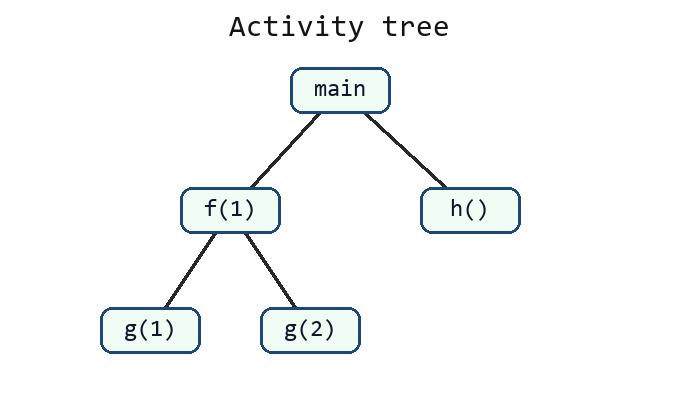
\includegraphics[width=0.82\linewidth]{figures/activity-tree-main-f-g-h.png}
\par{\small 活动树}
\end{figure}

子结点从左到右就是实际调用顺序。调用发生在进入过程时，所以调用顺序是活动树的前序遍历：

\begin{Verbatim}[fontsize=\small,breaklines=true]
main -> f(1) -> g(1) -> g(2) -> h()
\end{Verbatim}

\paragraph*{3. 过程返回顺序}

一个过程必须等它调用的子过程全部返回后才能返回，所以返回顺序是后序遍历：

\begin{Verbatim}[fontsize=\small,breaklines=true]
g(1) -> g(2) -> f(1) -> h() -> main
\end{Verbatim}

\paragraph*{4. 位于 `g(2)` 内部时的控制栈}

执行到 \texttt{g(2)} 时，\texttt{g(1)} 已经返回，\texttt{h()} 尚未调用。

\begin{longtable}{|p{0.47\linewidth}|p{0.47\linewidth}|}
\hline
活动 & 状态 \\
\hline
\endfirsthead
活动 & 状态 \\
\hline
\endhead
main & 已调用，尚未结束 \\
\hline
f(1) & 已调用，尚未结束 \\
\hline
g(1) & 已返回 \\
\hline
g(2) & 当前正在执行 \\
\hline
h() & 尚未调用 \\
\hline
\end{longtable}

因此尚未结束的活动是：

\begin{Verbatim}[fontsize=\small,breaklines=true]
main, f(1), g(2)
\end{Verbatim}

控制栈从栈底到栈顶为：

\begin{Verbatim}[fontsize=\small,breaklines=true]
AR(main), AR(f(1)), AR(g(2))
\end{Verbatim}

\paragraph*{5. 活动树遍历与调用/返回顺序}

\begin{longtable}{|p{0.47\linewidth}|p{0.47\linewidth}|}
\hline
遍历 & 对应含义 \\
\hline
\endfirsthead
遍历 & 对应含义 \\
\hline
\endhead
前序遍历 & 先访问当前结点，再访问子结点；对应过程调用顺序 \\
\hline
后序遍历 & 先访问子结点，再访问当前结点；对应过程返回顺序 \\
\hline
\end{longtable}

当前控制栈对应活动树中“根结点到当前活动结点”的路径。

\subsubsection*{二、栈帧布局与调用/返回答案}

\paragraph*{1. 从压入参数到完成函数序言的指令顺序}

题目约定参数从右到左压栈。调用 \texttt{fun(i,j)} 时，右侧参数 \texttt{j} 对应形参 \texttt{b}，左侧参数 \texttt{i} 对应形参 \texttt{a}。

\begin{Verbatim}[fontsize=\small,breaklines=true]
push j          ; 压入参数 b=20
push i          ; 压入参数 a=100
call fun        ; 压入返回地址，并跳转到 fun

fun:
push BP         ; 保存 main 的旧 BP
mov  BP, SP     ; 令 BP 指向刚压入的旧 BP
sub  SP, 4      ; 为局部变量 c 分配 4 字节
\end{Verbatim}

执行 \texttt{push BP} 后，栈顶位置保存的是旧 BP；随后 \texttt{BP=SP}，所以旧 BP 位于 \texttt{[BP+0]}。

\paragraph*{2. 以 BP 为基准的偏移}

题目约定机器字长 4 字节，栈向低地址增长。完成函数序言后布局如下：

\begin{figure}[H]\centering
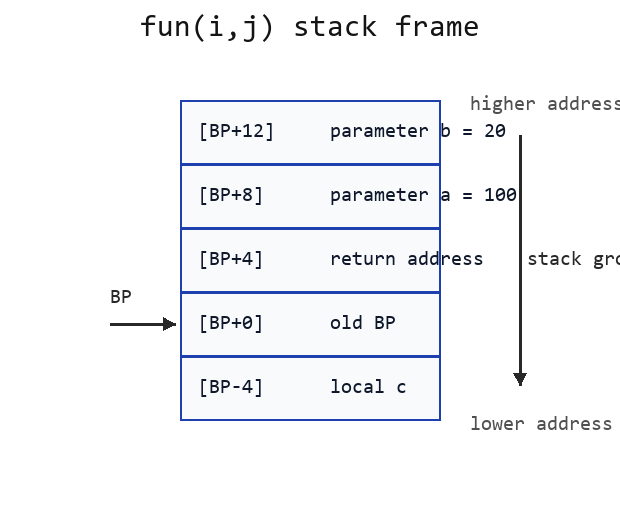
\includegraphics[width=0.82\linewidth]{figures/stack-frame-fun.png}
\par{\small fun(i,j) 栈帧布局}
\end{figure}

\begin{longtable}{|p{0.31\linewidth}|p{0.31\linewidth}|p{0.31\linewidth}|}
\hline
位置 & 内容 & 原因 \\
\hline
\endfirsthead
位置 & 内容 & 原因 \\
\hline
\endhead
\texttt{[BP-4]} & 局部变量 \texttt{c} & \texttt{sub SP,4} 在 BP 下方分配 4 字节 \\
\hline
\texttt{[BP+0]} & 旧 BP & \texttt{push BP} 后立刻 \texttt{BP=SP} \\
\hline
\texttt{[BP+4]} & 返回地址 & \texttt{call fun} 压入 \\
\hline
\texttt{[BP+8]} & 参数 \texttt{a=100} & 调用者后压入 \texttt{i}，离返回地址更近 \\
\hline
\texttt{[BP+12]} & 参数 \texttt{b=20} & 调用者先压入 \texttt{j}，位置更高 \\
\hline
\end{longtable}

\paragraph*{3. `c=a-b` 和设置返回值}

\begin{Verbatim}[fontsize=\small,breaklines=true]
LD   R0, [BP+8]       ; R0 = a = 100
SUB  R0, [BP+12]      ; R0 = a - b = 80
ST   [BP-4], R0       ; c = 80
LD   R0, [BP-4]       ; 返回值放入 R0
\end{Verbatim}

也可以在 \texttt{SUB} 后直接把 \texttt{R0} 作为返回值；这里按题目中的局部变量 \texttt{c} 明确写出存储和读取。

\paragraph*{4. 函数尾声和返回过程}

\begin{Verbatim}[fontsize=\small,breaklines=true]
mov  SP, BP           ; 释放局部变量 c
pop  BP               ; 恢复调用者 BP
ret                   ; 弹出返回地址并跳回 main
\end{Verbatim}

解释：

\begin{longtable}{|p{0.47\linewidth}|p{0.47\linewidth}|}
\hline
指令 & 作用 \\
\hline
\endfirsthead
指令 & 作用 \\
\hline
\endhead
\texttt{mov SP,BP} & SP 回到旧 BP 所在位置，局部变量空间失效 \\
\hline
\texttt{pop BP} & 取出旧 BP，恢复 main 的栈帧基址 \\
\hline
\texttt{ret} & 取出返回地址，跳回调用点之后 \\
\hline
\end{longtable}

\paragraph*{5. `main` 如何得到 `m=80`}

\texttt{fun} 返回时，返回值已经放在 \texttt{R0}。回到 \texttt{main} 后，调用者清理参数并保存返回值：

\begin{Verbatim}[fontsize=\small,breaklines=true]
add SP, 8             ; 清理两个 4 字节参数
ST  m, R0             ; m = 80
\end{Verbatim}

因此 \texttt{main} 中的 \texttt{m} 得到 \texttt{80}。

\subsubsection*{三、堆分配、碎片与分配策略答案}

\paragraph*{1. First-Fit}

First-Fit 从低地址到高地址扫描，选择第一个能满足请求的空闲块。

初始：

\begin{Verbatim}[fontsize=\small,breaklines=true]
[6, 14, 8, 20]
\end{Verbatim}

\begin{longtable}{|p{0.31\linewidth}|p{0.31\linewidth}|p{0.31\linewidth}|}
\hline
请求 & 扫描选择 & 分配后空闲块 \\
\hline
\endfirsthead
请求 & 扫描选择 & 分配后空闲块 \\
\hline
\endhead
7 & 6 不够，14 够，从 14 中切出 7 & \texttt{[6, 7, 8, 20]} \\
\hline
5 & 第一个块 6 够，从 6 中切出 5 & \texttt{[1, 7, 8, 20]} \\
\hline
12 & 1、7、8 不够，20 够，从 20 中切出 12 & \texttt{[1, 7, 8, 8]} \\
\hline
\end{longtable}

最终空闲块大小：

\begin{Verbatim}[fontsize=\small,breaklines=true]
[1, 7, 8, 8]
\end{Verbatim}

\paragraph*{2. Best-Fit}

Best-Fit 选择所有可满足请求的块中最小的那个。

\begin{longtable}{|p{0.23\linewidth}|p{0.23\linewidth}|p{0.23\linewidth}|p{0.23\linewidth}|}
\hline
请求 & 可选块 & 选择 & 分配后空闲块 \\
\hline
\endfirsthead
请求 & 可选块 & 选择 & 分配后空闲块 \\
\hline
\endhead
7 & 14, 8, 20 & 8 & \texttt{[6, 14, 1, 20]} \\
\hline
5 & 6, 14, 20 & 6 & \texttt{[1, 14, 1, 20]} \\
\hline
12 & 14, 20 & 14 & \texttt{[1, 2, 1, 20]} \\
\hline
\end{longtable}

最终空闲块大小：

\begin{Verbatim}[fontsize=\small,breaklines=true]
[1, 2, 1, 20]
\end{Verbatim}

\paragraph*{3. 最大连续空闲块比较}

\begin{longtable}{|p{0.31\linewidth}|p{0.31\linewidth}|p{0.31\linewidth}|}
\hline
策略 & 最终空闲块 & 最大连续空闲块 \\
\hline
\endfirsthead
策略 & 最终空闲块 & 最大连续空闲块 \\
\hline
\endhead
First-Fit & \texttt{[1,7,8,8]} & 8 \\
\hline
Best-Fit & \texttt{[1,2,1,20]} & 20 \\
\hline
\end{longtable}

本题给定请求序列下，Best-Fit 最终留下的最大连续空闲块更大。

\paragraph*{4. 内部碎片和外部碎片}

\begin{longtable}{|p{0.31\linewidth}|p{0.31\linewidth}|p{0.31\linewidth}|}
\hline
碎片类型 & 定义 & 例子 \\
\hline
\endfirsthead
碎片类型 & 定义 & 例子 \\
\hline
\endhead
内部碎片 & 已分配块内部没有被实际使用的空间 & 请求 13，但按 16 字节块分配，浪费 3 \\
\hline
外部碎片 & 空闲空间总量足够，但分散成多个不连续小块 & 空闲 5+5+5，总量 15，但无法满足连续 12 的请求 \\
\hline
\end{longtable}

\paragraph*{5. 存储管理器评价维度}

\begin{longtable}{|p{0.47\linewidth}|p{0.47\linewidth}|}
\hline
维度 & 含义 \\
\hline
\endfirsthead
维度 & 含义 \\
\hline
\endhead
空间效率 & 降低碎片和总堆占用 \\
\hline
程序效率 & 分配布局有利于访问局部性和缓存 \\
\hline
低开销 & 分配、释放、回收、维护元数据的成本低 \\
\hline
\end{longtable}

\subsubsection*{四、引用计数与不可达环答案}

对象图如下：

\begin{figure}[H]\centering
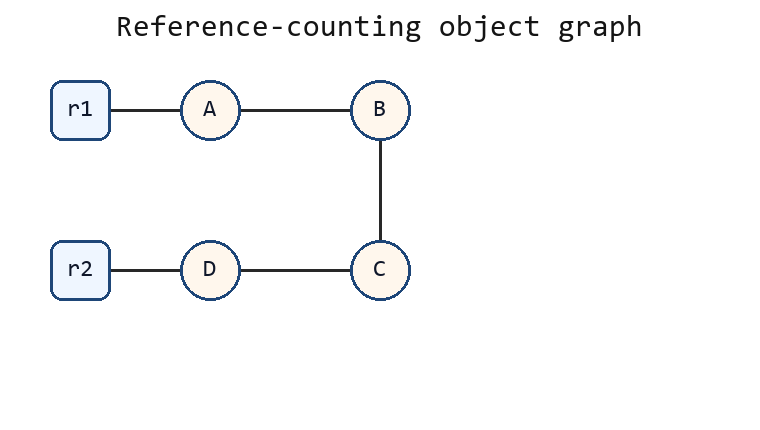
\includegraphics[width=0.82\linewidth]{figures/rc-object-graph.png}
\par{\small 引用计数对象图}
\end{figure}

\paragraph*{1. 初始引用计数}

引用来源：

\begin{Verbatim}[fontsize=\small,breaklines=true]
r1 -> A
r2 -> D
A  -> B
B  -> C
C  -> B
D  -> C
\end{Verbatim}

\begin{longtable}{|p{0.31\linewidth}|p{0.31\linewidth}|p{0.31\linewidth}|}
\hline
对象 & 入边来源 & 初始 RC \\
\hline
\endfirsthead
对象 & 入边来源 & 初始 RC \\
\hline
\endhead
A & r1 & 1 \\
\hline
B & A, C & 2 \\
\hline
C & B, D & 2 \\
\hline
D & r2 & 1 \\
\hline
\end{longtable}

\paragraph*{2. 执行 `r1=null`}

\texttt{r1} 不再指向 A：

\begin{Verbatim}[fontsize=\small,breaklines=true]
RC(A): 1 -> 0
\end{Verbatim}

A 被回收。回收 A 时删除 A 的出边 \texttt{A -> B}：

\begin{Verbatim}[fontsize=\small,breaklines=true]
RC(B): 2 -> 1
\end{Verbatim}

此时：

\begin{longtable}{|p{0.47\linewidth}|p{0.47\linewidth}|}
\hline
对象 & RC \\
\hline
\endfirsthead
对象 & RC \\
\hline
\endhead
B & 1 \\
\hline
C & 2 \\
\hline
D & 1 \\
\hline
\end{longtable}

\paragraph*{3. 再执行 `r2=null`}

\texttt{r2} 不再指向 D：

\begin{Verbatim}[fontsize=\small,breaklines=true]
RC(D): 1 -> 0
\end{Verbatim}

D 被回收。回收 D 时删除 D 的出边 \texttt{D -> C}：

\begin{Verbatim}[fontsize=\small,breaklines=true]
RC(C): 2 -> 1
\end{Verbatim}

此时：

\begin{longtable}{|p{0.47\linewidth}|p{0.47\linewidth}|}
\hline
对象 & RC \\
\hline
\endfirsthead
对象 & RC \\
\hline
\endhead
B & 1 \\
\hline
C & 1 \\
\hline
\end{longtable}

\paragraph*{4. 不可达但不能被引用计数回收的对象}

根 \texttt{r1}、\texttt{r2} 都为 null 后，根集已经无法到达 B 和 C。但 B 和 C 互相引用：

\begin{Verbatim}[fontsize=\small,breaklines=true]
B -> C
C -> B
\end{Verbatim}

所以：

\begin{Verbatim}[fontsize=\small,breaklines=true]
RC(B)=1
RC(C)=1
\end{Verbatim}

它们都不是 0，引用计数不会触发回收。不可达但不能被引用计数回收的对象是：

\begin{Verbatim}[fontsize=\small,breaklines=true]
B, C
\end{Verbatim}

\paragraph*{5. 跟踪式垃圾回收为什么能回收}

跟踪式 GC 从根集出发，只标记从根可达的对象。此时根集为空或不指向 B/C，因此 B、C 不会被标记。清扫阶段回收所有未标记对象，所以能回收不可达环。

\subsubsection*{五、标记-清扫、压缩、拷贝与分代答案}

对象图如下：

\begin{figure}[H]\centering
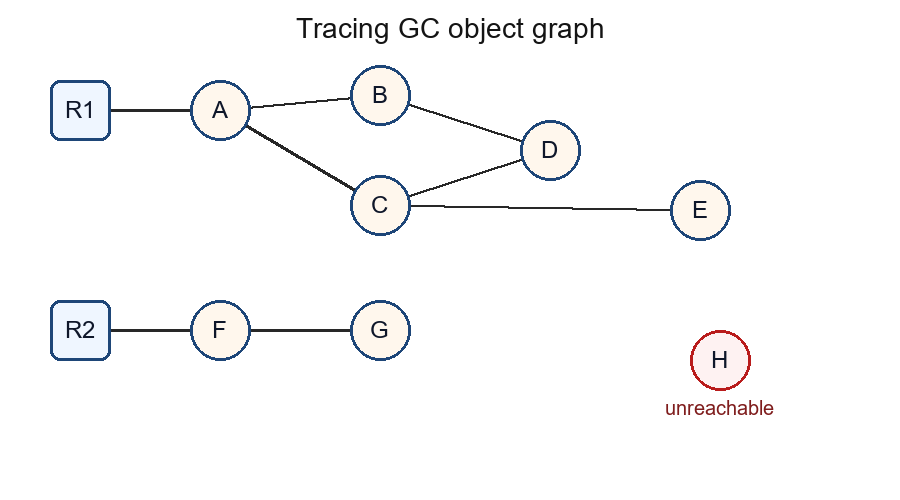
\includegraphics[width=0.82\linewidth]{figures/trace-object-graph.png}
\par{\small 标记-清扫对象图}
\end{figure}

\paragraph*{1. 可达对象和垃圾对象}

从根出发：

\begin{Verbatim}[fontsize=\small,breaklines=true]
R1 -> A -> B -> D
R1 -> A -> C -> D
R1 -> A -> C -> E
R2 -> F -> G
\end{Verbatim}

可达集合：

\begin{Verbatim}[fontsize=\small,breaklines=true]
{A, B, C, D, E, F, G}
\end{Verbatim}

垃圾对象：

\begin{Verbatim}[fontsize=\small,breaklines=true]
{H}
\end{Verbatim}

\paragraph*{2. 标记-清扫过程}

\begin{longtable}{|p{0.47\linewidth}|p{0.47\linewidth}|}
\hline
阶段 & 操作 \\
\hline
\endfirsthead
阶段 & 操作 \\
\hline
\endhead
标记 & 从 R1、R2 出发遍历引用图，标记 A、B、C、D、E、F、G \\
\hline
清扫 & 线性扫描堆，发现 H 未标记，释放 H 的空间 \\
\hline
\end{longtable}

清扫后 H 的地址区间 \texttt{[2,4)} 成为空闲块。

\paragraph*{3. 压缩后的新地址}

按原有地址顺序保留存活对象，并向低地址压缩。H 被删除，后面的存活对象前移。

\begin{longtable}{|p{0.23\linewidth}|p{0.23\linewidth}|p{0.23\linewidth}|p{0.23\linewidth}|}
\hline
对象 & 旧起始地址 & 大小 & 新起始地址 \\
\hline
\endfirsthead
对象 & 旧起始地址 & 大小 & 新起始地址 \\
\hline
\endhead
A & 0 & 2 & 0 \\
\hline
B & 4 & 3 & 2 \\
\hline
C & 7 & 2 & 5 \\
\hline
D & 9 & 1 & 7 \\
\hline
E & 10 & 2 & 8 \\
\hline
F & 12 & 1 & 10 \\
\hline
G & 13 & 2 & 11 \\
\hline
\end{longtable}

压缩后存活对象占用连续区间：

\begin{Verbatim}[fontsize=\small,breaklines=true]
[0, 13)
\end{Verbatim}

所有根和对象字段中的旧地址都必须更新为新地址。

\paragraph*{4. 半空间拷贝回收}

半空间拷贝把堆分成 From 和 To 两个半空间：

\begin{longtable}{|p{0.47\linewidth}|p{0.47\linewidth}|}
\hline
阶段 & 动作 \\
\hline
\endfirsthead
阶段 & 动作 \\
\hline
\endhead
正常分配 & 只在 From 空间中顺序分配 \\
\hline
回收开始 & 从根出发，把可达对象复制到 To 空间 \\
\hline
更新引用 & 用复制后的新地址更新根和对象字段 \\
\hline
回收结束 & 交换 From 和 To；旧 From 中未复制对象自然被丢弃 \\
\hline
\end{longtable}

空间代价：同一时刻通常只有一半堆空间用于分配，因为另一半要作为 To 空间。

\paragraph*{5. 分代回收与记忆集}

分代回收依据经验规律：

\begin{Verbatim}[fontsize=\small,breaklines=true]
多数对象很快死亡，少数对象存活很久。
\end{Verbatim}

因此把堆分为新生代和老年代：

\begin{longtable}{|p{0.47\linewidth}|p{0.47\linewidth}|}
\hline
区域 & 回收特点 \\
\hline
\endfirsthead
区域 & 回收特点 \\
\hline
\endhead
新生代 & 容量较小，回收频繁 \\
\hline
老年代 & 存活时间长，回收频率低 \\
\hline
\end{longtable}

记忆集记录“老年代对象指向新生代对象”的引用。回收新生代时，除了栈和全局变量等根，还要把记忆集中的引用当作额外根，这样不用扫描整个老年代。
\end{document}
